\section{以双平方根方程实现观测排列延拓}
\label{sec:3.3}
本节将讨论用一种更广泛意义的成像概念,即观测排列延拓\footnote{原文为experiment
sinking,若按字面直接译出,其意义不易明瞭,现根据该概念的实际意又,按现已习惯通用
的术语译为“观测排列延拓”--译者}来取代爆炸反射面成像概念,将建立一种称为双平方根方程(DSR
)的新方程来实现观测排列延拓成像。DSR方程的
作用就是将整个地震勘探排列向下延拓,不单只是检波点向下延拓,而且炮点也向下延拓。
在导出DSR方程之后,本章其余部份将专门致力于用DSR方程来解释偏移、叠加、叠前偏
移、速度分析及横向速度变化的校正等问题。

瞧一眼前面的式\ref{eq:ex3.2.9},你就会发现这是一种具有两个平方根的方程。一个平方根
项代表波到达角的余弦,另一个平方根项代表炮点上的出射角之余弦;一个余弦项可以用沿
$(s,g,t)$空间内检波点所在坐标轴之Fourier分量$k_g$来表示,另一项余弦可用沿炮点所
在坐标轴之Fourier分量$k_s$来表示。

野外地震记录位于$(s,g)$平面内,为转移至地震解释人员所习惯的$(y,h)$
平面,只需作简单的旋转即可,这样就可沿$y$和$h$将资料作Fourier变换,然后就能用本节的式
\ref{eq:ex3.3.17}、而不是用式\ref{eq:ex3.3.9}来进行向下延拓的处理。

DSR方程与互换原理有关,我们首先要回顾一下该原理。

\subsection{地震互换原理及其应用}
\label{sec:3.3.1}

互换原理是说:如果震濂与检波器互换位置,所得地震记录应相同。互换性得以成立的
物理原因就在于:不论观测排列如何复杂,沿射线的波速在任一方向上均相同。

从数学上说,出现互换性原理是因为弹性物理方程是属于自伴随(self adjoint
)的自伴随这一术语的意义在《地震数据处理基础》一书中有所解释,书中指出,业经离散化后
的声波方程形成一个对称矩阵,即使密度与压缩系数均属空间可变时亦如此;任何此类矩阵
之逆仍是另一种称作脉冲响应矩阵的对称矩阵,相对于该矩阵对角线前各元素均彼此相等;
任何一对元素中,每个元素都是对脉冲源的响应,这成对相向的两个元素就涉及到被互换的
源与接收点。

关于互换性有一件棘手的事情就是必须妥善处理方向特性作用。例如,单个的垂直检波
器本身就有一种天然的方向特性,它既不可能接收水平传播的压力波,也不可能接收垂直传
播的剪切波。为使互换性得以应用,当震源与接收点互换时,必须使方向特性保持不变,方
向特性必须认为是介质所固有的,不因检波器而变化。

\begin{figure}[H]
\centering
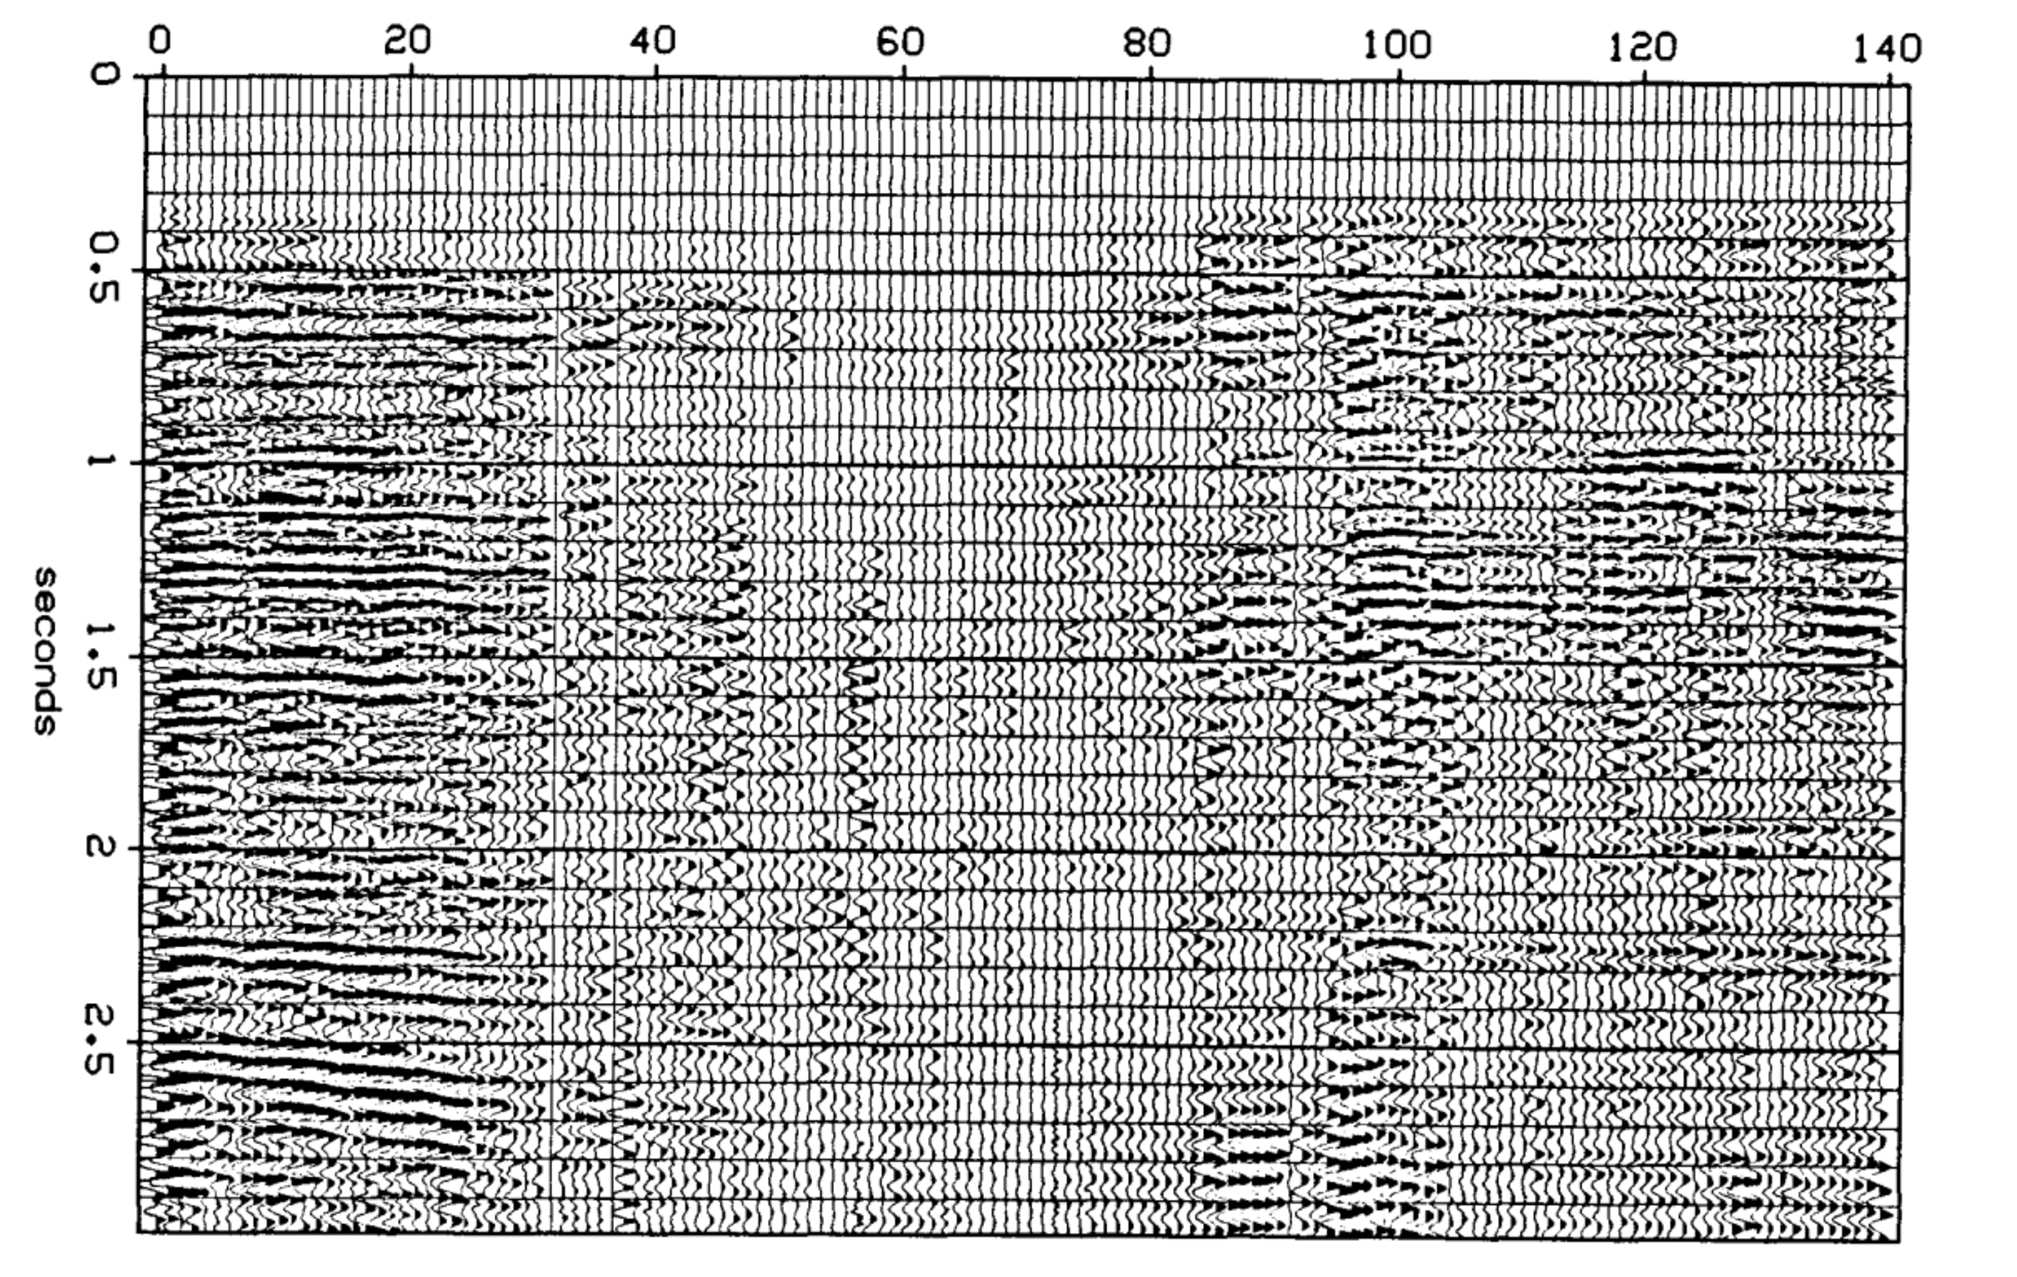
\includegraphics[width=0.65\textwidth]{ofs/chervon}
\caption[chervon]{加利福尼亚Central Valley地区的共炮检距时间剖面}
\label{fig:ofs/chervon}
\end{figure}

从我们的数据库中我查出一种能说明野外观测条件下之互换性的中间放炮排列陆地资
料。图\ref{fig:ofs/chervon}所示共炮检距时间剖面系采用垂直振动源和垂直检波器所记录,该项观测并非
专为检查互换性的目的而进行,所以炮点测线与接收点测线之间似乎有一点横向偏移;因类
似的原因,震源组合与检波器组合方式可能也稍微有点不同,虽然已经知道横向速度变化是
该地区的一个问题,可是图\ref{fig:ofs/chervon}中的地层倾角却恰好相当小。

图\ref{fig:ofs/reciptrace}所绘是三个互换地震记录的开始部分,分别为近炮检距、中等炮检距及远炮检
距上所选之成对记录。你能看出,各互换地震记录一般均具有相同极性,而且往往具有近乎
相等的振幅(该图所示系图\ref{fig:ofs/chervon}中最好的三个记录)。
\begin{figure}[H]
\centering
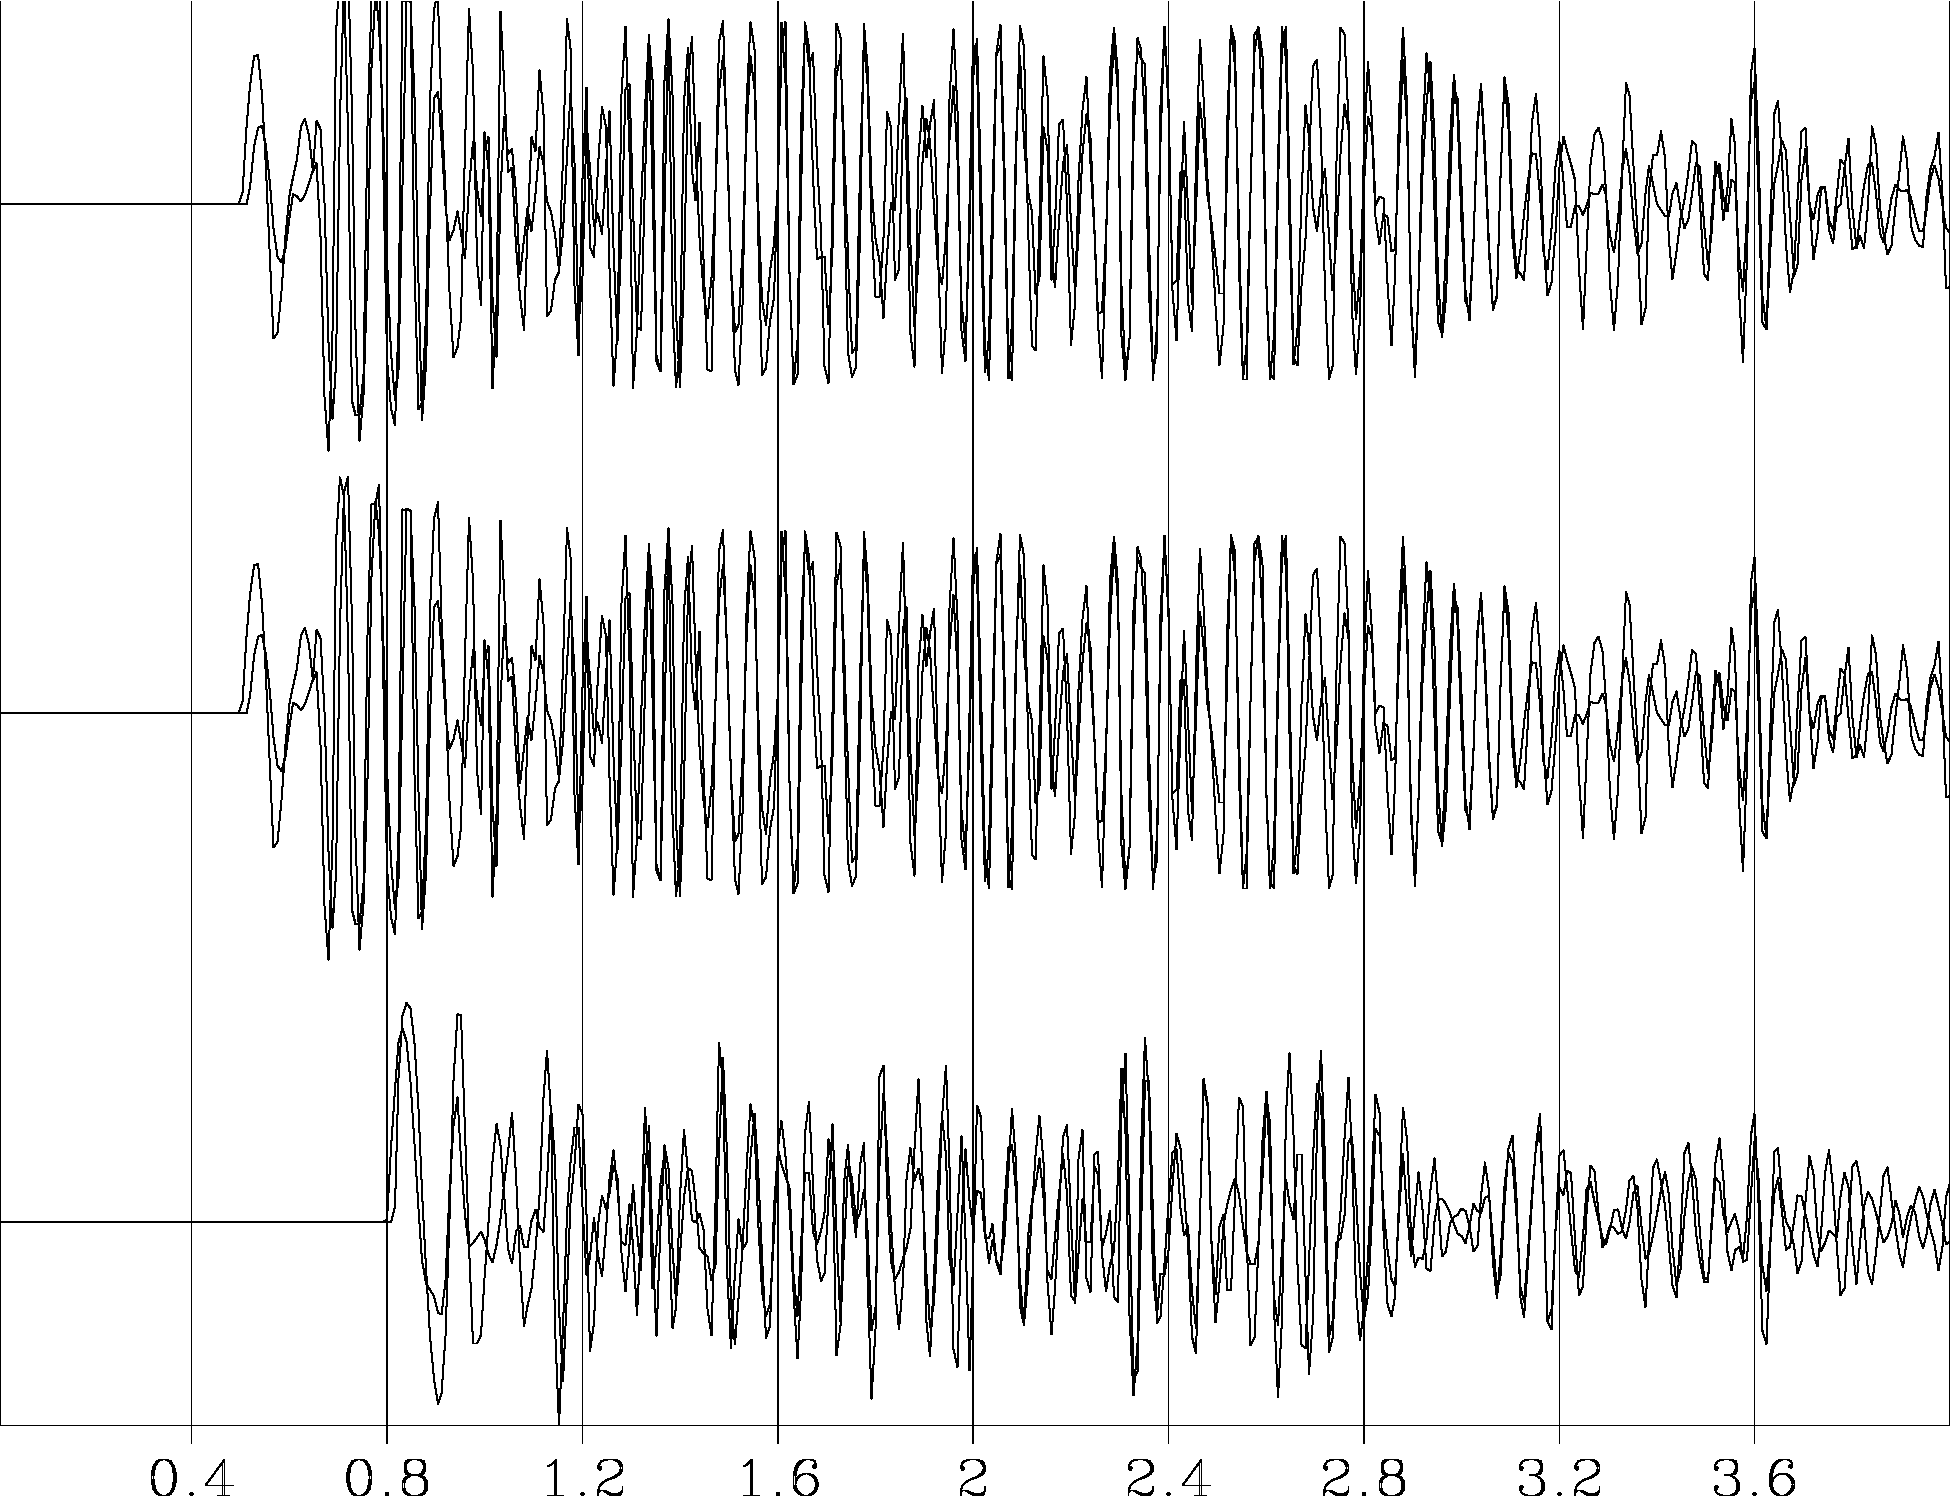
\includegraphics[width=0.65\textwidth]{ofs/reciptrace}
\caption[reciptrace]{重叠的互换地震记录}
\label{fig:ofs/reciptrace}
\end{figure}

\begin{figure}[H]
\centering
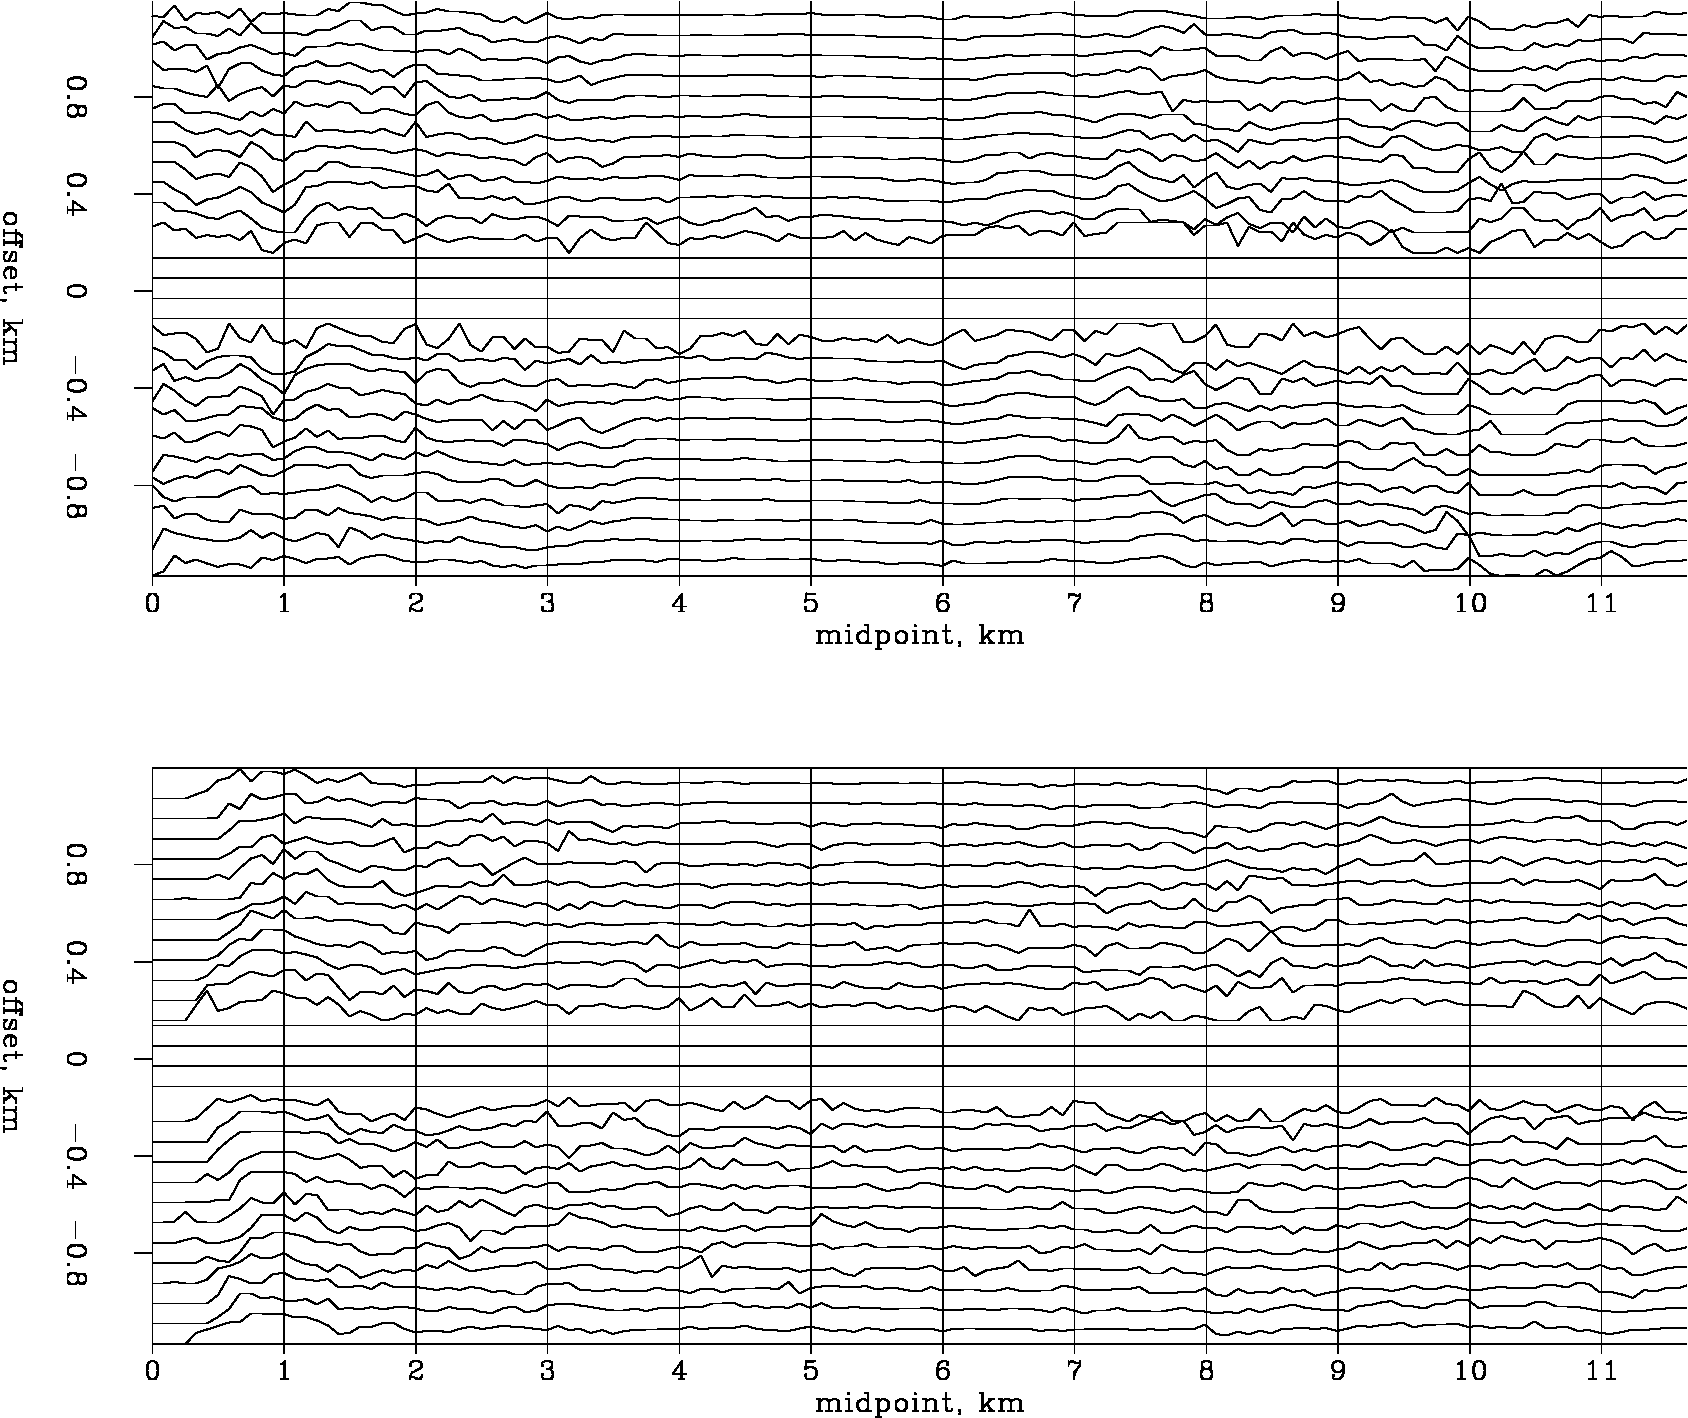
\includegraphics[width=0.65\textwidth]{ofs/recipslice}
\caption[recipslice]{1s与2.5s处的恒定时间切片}
\label{fig:ofs/recipslice}
\end{figure}

图\ref{fig:ofs/recipslice}中的各个恒定时间切片表明许多成对地震记录的互换性,该图所涉及的中心点
水平距离范围与图\ref{fig:ofs/chervon}相同,垂直坐轴则表示炮检距。该项资料不是在振动器附近所记
录,所以使中心部分留有空隙。为使不相干变化极小,动校正是在作时间切片之前完成的
(图左端呈现缺炮的影响)。由图\ref{fig:ofs/recipslice}那样的切片所组成的一系列连续画面有一种特点,即
是:你在各别画面中所见到的左右对称性是所有时间上的共同特征。不过要注意,在号
中心点附近的1秒时间切片上却是显著偏离互换性要求的。

在实验室中,可在观测精度限度内证实互换性的存在,这可能是最佳结果了
(见《地震数搪处理基础》一书中所举White所作的实验例子)。在野外环境下,互换性是否有效依赖于所
要求条铧能被满足至何种程度。海上勘探所甩空气枪应是可与水听器互换的;地面重锤震源
应是可与垂直检波器互换的,但是地下爆炸炮点却并不一定与地面垂直检波器是可互换的,
因为二者方向特性不同,而且二者位置亦稍有不同。 Fenati与Rocca(1984)曾研究过野
外变动条件下的互换性问题,他们报道过震源与接收器的微小定位误差可以很容易形成比视
互换性差异还大的偏差;他们也曾报道过,理论的互换性观测排列实际上也许比假想的非互
换性观测排列还缺乏互换性。

地层内部几何形态的复杂性并未降低线性原理应用的可能,与此类似,几何复杂性并未
使互换性难于应用,在有风的情况下,不能把互换性应用于声波,因为声波在迎风时比顺风
时要传播得慢一些。但是比起野外工作中普遍常见的各种不规则性来,风的这种影响就是非
常微不足道了。仅只是由于反射随时间而衰减这一项,就要使不具互换性的干扰噪音变得突
出起来。往后我们将假设,互换性一般是可应用于反射地震资料分析的。

\subsection{观测排列延拓概念}
\label{sec:3.3.2}

爆炸反射面概念有很大用处,因为它能使我们把许多观测排列内(比如说,多达1000个
炮点)在零炮检距上所观测到的地震波同一个假想观测排列的波联系起来,即与爆炸反射面
观测记录结果联系起来。对爆炸反射面的模拟类比,有几个关系到横向速度变化与多次反射
的公认限制。一个主要限制是:爆炸反射面概念没有向我们提供关于非零炮检距记录资料究
应如何进行偏移的任何线索,所以,需要有更广泛意义上的成像概念才行。

就从测线是沿欠坐标轴分布的野外资料开始说起吧。设有无限多观测排列。一个观测排
列是指:点震源或炮点置于$x$轴上的$s$处,然后用轴上各个可能位置$g$上分布的检波器对反射
进行记录。所以,观测到的资料是一种上行波,它是与$s$和$g$有关的二维函数$P(s,g,t)$
。(有关炮点与检波点的实际间距与分布范围等重要的应用问题,将推迟至\ref{sec:3.6}节和\ref{sec:4.3}节再讨论)。

以前几章已经指出如何使上行波向下延拓。上行波的向下延拓实际上与检波点的向下延
拓是一回事,完全不涉及震源点的延拓处理。上行波可以从一个爆炸反射面开始,或者可以
在地面开始,向下进行,然后向上反射回去。

为应用观测排列延拓的成像概念,就有必要不但使检波点向下延拓,而且也要使震滙向
下延拓,我们已经知道如何使检波点向下延拓了,由于互换性允许检波点与炮点相互交换,
所以实际上我们也就是知道了如何将炮点向下延拓了。

炮点与检波点可以向下延拓至不同的深度水平,因而在这种处理中间,它们可以处于不
同深度水平,不过就最终处理结果要求来说,仅需要它们处在相同深度水平;这就是说,取
$z_s$为炮点深度和$z_g$为检波点深度时,向下延拓处理将要求在所有水平上都是$z=z_s=s_g$

位于$(x,z)$的反射面之映像是按最靠近的可能的成对炮点与检波点上所见到的反射强
度与极性来定义的,取其数学极限时,这种最靠近的成对点相当于震源与检波点在反射面上
彼此重合了,这时的反射旅行时间等于零。这种观测排列延拓成像概念可总结为下列关系:
